\documentclass[tikz,border=5pt]{standalone}
\usepackage{tikz}
\usetikzlibrary{positioning,calc}

\begin{document}
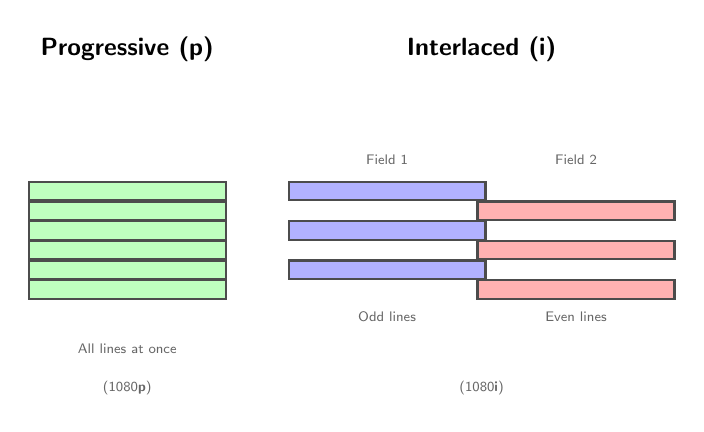
\begin{tikzpicture}[
    line/.style={draw=black!70, thick, minimum width=2.5cm, minimum height=0.15cm},
    oddline/.style={line, fill=blue!30},
    evenline/.style={line, fill=red!30},
    fullline/.style={line, fill=green!25},
    label/.style={font=\small\sffamily\bfseries},
    sublabel/.style={font=\tiny\sffamily, text=black!60}
]

% Progressive
\begin{scope}[shift={(0,0)}]
    \node[label] at (0, 1.8) {Progressive (p)};

    \foreach \i in {0,...,5} {
        \node[fullline] at (0, -\i*0.25) {};
    }

    \node[sublabel] at (0, -2.0) {All lines at once};
    \node[sublabel] at (0, -2.5) {(1080\textbf{p})};
\end{scope}

% Interlaced
\begin{scope}[shift={(4.5,0)}]
    \node[label] at (0, 1.8) {Interlaced (i)};

    % Field 1 (odd)
    \begin{scope}[shift={(-1.2,0)}]
        \node[sublabel] at (0, 0.4) {Field 1};
        \node[oddline] at (0, 0) {};
        \node[oddline] at (0, -0.5) {};
        \node[oddline] at (0, -1.0) {};
        \node[sublabel] at (0, -1.6) {Odd lines};
    \end{scope}

    % Field 2 (even)
    \begin{scope}[shift={(1.2,0)}]
        \node[sublabel] at (0, 0.4) {Field 2};
        \node[evenline] at (0, -0.25) {};
        \node[evenline] at (0, -0.75) {};
        \node[evenline] at (0, -1.25) {};
        \node[sublabel] at (0, -1.6) {Even lines};
    \end{scope}

    \node[sublabel] at (0, -2.5) {(1080\textbf{i})};
\end{scope}

\end{tikzpicture}
\end{document}
